\chapter{Energy Landscapes}
\label{ch:energy_landscapes}
\graphicspath{{energy_landscapes/fig/}}

This chapter aims to introduce key concepts in the theory of energy landscapes and how they can be utilised.
These include definitions of salient critical points in the energy landscapes of interest in this thesis.
Then, a summary is provided for some of the various applications to which they have been used.


\section{Features of energy landscapes}
\begin{figure}
  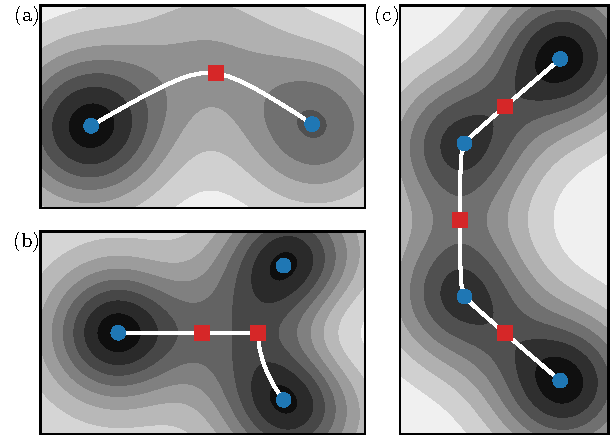
\includegraphics{features.pdf}
  \caption{\label{fig:el-features}
    Schematics showing 2D energy landscapes with the features of interest.
    Blue circles represent the minima, red squares show the transition states, and white paths show the MEPs.
    (a) A simple landscape with two minima connected by a single MEP.
    (b) A landscape where an MEP should terminate at a transition state.
        However, running downhill from the left-most transition state goes past this and continues to a minimum.
    (c) A multi-step pathway with two intermediate minima.
        The full MEP between the top and bottom minima is a combination of the three individual MEPs.
  }
\end{figure}
An energy landscape describes how the energy of a system changes throughout its configuration space.
These are often very high-dimensional landscapes, as the total number of degrees of freedom are typically very large, particularly when modelling continuous macroscale systems.

The primary points of interest are the stable states.
These correspond to local minima in the energy landscape, as any small perturbation would raise the energy and result in a driving force restoring it back to the minimum.
Mathematically, the energy in the vicinity of a minimum at $\bm{x}_0$ can be expressed as,
\begin{equation}
  E(\bm{x}) = E(\bm{x}_0) + \sum_i \frac{a_i}{2} \left. \frac{\partial^2 E}{\partial x_i^2} \right|_{\bm{x}_0} (x_i - x_{0,i})^2,
  \label{eq:el-criticalpoint}
\end{equation}
where $i$ represents each of the principal directions of curvature, and all of the curvatures, $a_i$, are positive.
Using energy minimisation methods to identify these stable states is central to the exploration of energy landscapes.
As an example, \cref{fig:el-features}(a) shows a 2D landscape containing two minima, as well as highlighting other features of interest.

Each minimum also possesses a basin of attraction, which is the surrounding region of points that will converge to the minimum upon following the gradient downhill.
Taking the analogy of a mountainous landscape, these basins correspond to valleys for which the dividing lines are ridges and watersheds.
The energy depth and the extent of a basin can be used to quantify the stability of the state; the former providing the energy required by a interaction to change the state, while the latter provides the required perturbation size.

Transition states (TS) are first-order saddle points on the energy landscape.
These are stationary points where the energy is defined by \cref{eq:el-criticalpoint} with a single negative curvature, $a_1 < 0$, while all others are positive or zero, $a_{i>1} \ge 0$.
These correspond to minima on the ridges separating basins of attraction, so they provide the lowest possible energy required to swap between two stable states.
This energy barrier is incredibly useful for quantifying the stability of states and the probability of a transition between them \cite{Mokkonen2016}.
The energy barrier is also an important quantity to estimate transition times in microscale systems, such as chemical reactions, using transition state theory \cite{Truhlar1996}.
Each transition state also uniquely defines a possible reconfiguration pathway, known as the minimum energy pathway (MEP).

The MEP, $\bm{x}(s)$, connects the transition state to its adjacent minima by following the path of steepest descent from either side of the saddle point,
\begin{equation}
  \deriv{\bm{x}}{s} = \hat{\tau} = - \frac{\grad E(\bm{x})} {|\grad E(\bm{x})|}.
\end{equation}
Here the pathway parameter $s$ is the integrated path length, so the derivative is the unit tangent vector of the pathway.
Therefore, if a transition state has already been found it is a simple process to obtain the MEP.
An equivalent statement, that can provide a convergence criterion for pathway search algorithms, is that the local gradient has no component perpendicular to the direction of the pathway at all points on its length,
\begin{equation}
  \grad^\perp E(\bm{x}) = \grad E(\bm{x}) - (\bm{\hat{\tau}} \cdot \grad E(\bm{x})) \bm{\hat{\tau}} = 0.
  \label{eq:el-mep-convergence}
\end{equation}

Sometimes the precise MEP can end at a transition state rather than a minimum if the steepest-descent pathway reaches a bifurcation point \cite{Wales2004}.
A separate MEP then runs downhill from this to the minima (or to other transition states).
However, in practice, small deviations from the steepest pathway will cause a breaking of symmetry in both experiment and simulations, and it will proceed all the way to one of the minima.
An example of this is shown in \cref{fig:el-features}(b).
MEPs can also be obtained between states that are separated by intermediate minima.
In this case, the MEP will consist of the combination of the individual MEPs between each adjacent pair of minima, each passing over a separate transition state (\cref{fig:el-features}(c)).
Hence, it is possible to build up a network of pathways between adjacent minima to identify all possible reconfiguration pathways of a system.
A single pair of minima can also have multiple pathways between them, even if they are adjacent to one another.
These different pathways can often be difficult to locate and there can be a large number of them in a high-dimensional landscape.
However, the most important are those with the lowest energy and most direct, which are the most easily identifiable.

The MEPs that are located are time independent, providing no direct information about the dynamics along the pathway.
On one hand, this allows energy landscape methods to be more efficient than performing the corresponding dynamical simulations, such as molecular dynamics or finite element analysis, particularly in the case of rare event transitions with barriers larger than $k_\mathrm{B}T$ \cite{Passerone2001}.
On the other hand, the true pathway taken by the system will depend upon the force driving the transition, and inertial effects can cause it to deviate from the steepest descent pathway.
Therefore, the MEP instead provides an ideal pathway that is independent of the force driving the reconfiguration, and provides the average and most probable path that will be taken if driven by random forces or thermal noise \cite{E2007}.

\section{Visualising energy landscapes}
It can be difficult to visualise the high-dimensional landscapes, but one simple way of doing so is using disconnectivity graphs \cite{Wales2004}.
These have a vertical axis showing the energies of all the minima and the transition states with the minimum required energies that connect them.
Such visualisations are useful because they clearly separate the energy landscape into a hierarchy of groups of states according to the ease of reconfiguring between them.
Additionally, the system can be characterised according to the shape of the graph \cite{Wales1998}.
If the energy barriers are tall the system will be trapped it in a single state, and it is referred to as a glassy landscape.
In contrast, small barriers allow the system to easily explore the landscape.
This can be seen by contrasting \cref{fig:el-disconnectivity}(a) and \cref{fig:el-disconnectivity}(b).
Furthermore, the energy landscape may be funnel-shaped, in which case it can quickly converge to the global minimum (\cref{fig:el-disconnectivity}(b)), while for a flat landscape (\cref{fig:el-disconnectivity}(c)) the system is not biased toward any particular state.

\section{Free energy landscapes}
An important concept for characterising the behaviour of a system is that of free energy landscapes.
Until now the discussion has focused mainly upon potential energy landscapes which differ from free energy landscapes in a couple of key ways.
Firstly, while potential energy landscapes are high-dimensional and depend upon all coordinates of the system, free energy landscapes often involve averaging over the coordinates to produce a lower-dimensional system that represents the overall behaviour \cite{Wales2004}.
Also, the free energy includes information about the thermodynamic nature of the system, because separate minima in the potential energy can correspond to a single minimum in the free energy if it can freely swap between them.
Therefore, the free energy landscape changes depending upon the temperature.

\Cref{fig:el-disconnectivity}(d) shows an example of this for a particle cluster, where the potential energy landscape has been reduced to a two-dimensional free energy landscape.
These two order parameters are the potential energy, $V$, and a face-centered cubic packing order parameter, $Q_4$.
Although, in this example there are no free energy minima with high $Q_4$.
At a high temperature there is just a single minimum for high potential energy states, which correspond to a liquid phase.
As the temperature lowers another minimum appears with low potential energy, representing the crystallised structure.
At this point the liquid and crystal states are both stable.
Finally, at the lowest temperatures the liquid minimum disappears and the cluster will only be found in its highly ordered configuration.

This distinction between free and potential energy landscapes are important for microscale and particulate systems where thermal noise is sufficient for the system to spontaneously explore different states.
However, for macroscale systems, which this thesis primarily focusses upon, we are already dealing with effective free energy models that correspond to a thermodynamic average of microstates.
Although there may be some random perturbing effects, such as vibrations, we generally do not consider any further averaging of the states.
Therefore, for brevity, we will simply term our study as an exploration of energy landscapes.

\begin{figure}
  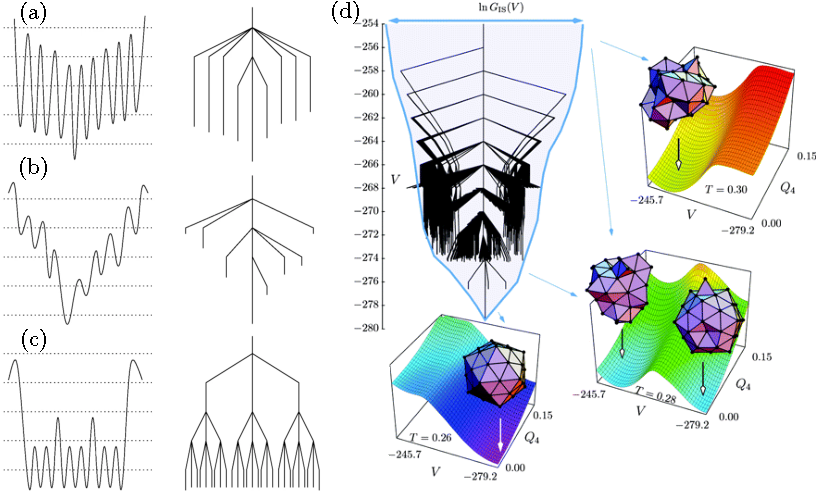
\includegraphics{disconnectivity}
  \caption{\label{fig:el-disconnectivity}
    (a-c) Disconnectivity graphs for three one-dimensional potentials, each exhibiting a different behaviour (see text for discussion).
    (d) Disconnectivity graph for a 55 particle cluster, with the envelope size representing the number of states at, or below, that energy.
        Three 2D free energy landscapes show the states of the system at different temperatures.
        Representative configurations are shown in each of the minima.
        Adapted with permission from \cite{Wales2006}.
  }
\end{figure}



\section{Applications of energy landscapes}
\begin{figure}
  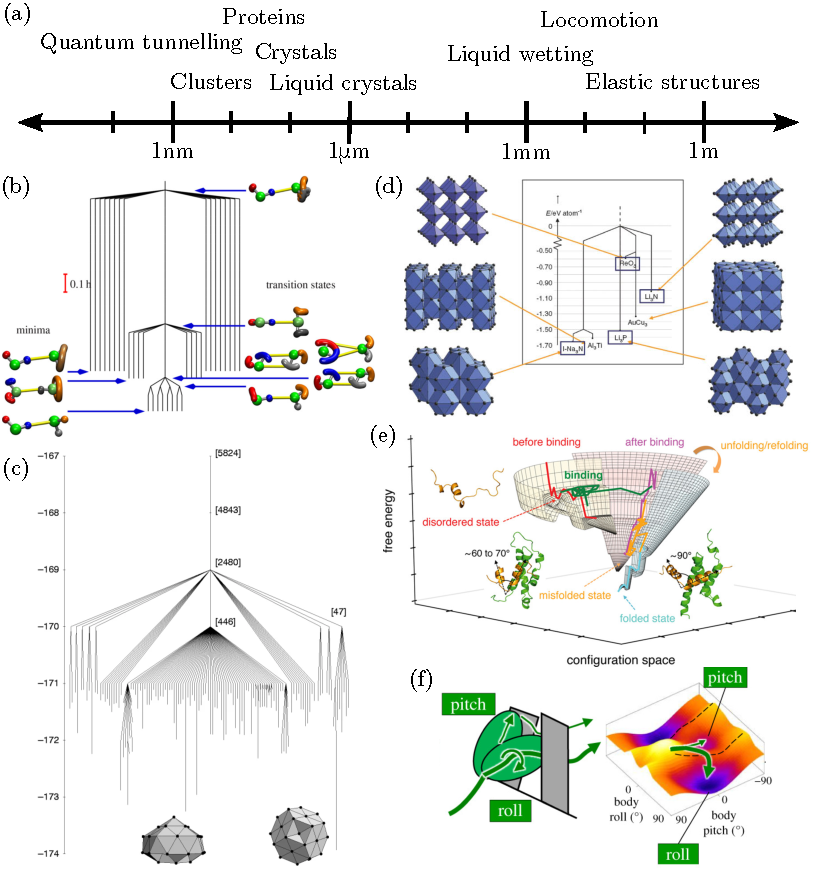
\includegraphics{applications}
  \caption{
    (a) Approximate length scales of various applications of energy landscapes techniques.
    (b) Energy landscape of a pair of hydrogen molecules where the transition states show instanton tunnelling pathways.
        Adapted with permission from \cite{Vaillant2019}.
    (c) Energy landscape showing the candidates for the crystal structure of $\mathrm{Na_3N}$.
        Adapted with permission from \cite{Jansen2014}.
    (d) Disconnectivity graph for a Lennard-Jones 38 particle cluster showing a large funnel for the native icosahedral structure, and a smaller funnel for the truncated octahedron structure.
        Adapted with permission from \cite{Wales1998}.
    (e) Energy landscape of an intrinsically disordered protein, pKID, that folds upon binding with another molecule.
        Adapted with permission from \cite{Chong2019}.
    (f) Diagram showing the two modes of locomotion to pass a barrier and the associate energy landscape.
        This shows the locomotor transition from the pitching to rolling motion.
        Adapted with permission from \cite{Othayoth2021}.
  }
  \label{fig:el-applications}
\end{figure}
Here, we will summarise known applications of energy landscape studies.
To illustrate their wide applicability, we will discuss phenomena across several orders of magnitude, from less than 1\si{nm} to larger than 1\si{m}.

To date, energy landscapes exploration techniques see their most prominent applications in particulate and molecular systems.
At the smallest scales, these are used to study the transition pathways of chemical reactions, where the stable states represent the reactants and products, as well as any reaction intermediates.
Such applications are the source of the term `transition state' which has particular importance for finding reaction rates according to transition state theory.

To obtain accurate chemical reaction rates it is often necessary to consider the effects of quantum tunnelling, which can cause transitions to occur that are classically disallowed.
It is possible to use information about energy barriers and MEP to provide tunnelling corrections to the classical rates from transition state theory \cite{Truhlar1971,Miller1979}.
However, quantum tunnelling depends upon the width of a barrier, not just its height, so shorter paths than the MEP may be more important for determining accurate tunnelling rates.
One approach is to use instantons, which are based upon the path integral formulation of quantum mechanics.
These provide a temperature-dependent pathway that `cuts the corner' of the MEP, providing a more direct path at the expense of a higher barrier \cite{Richardson2016,Richardson2018}.
By finding the transition states of these instantons the effective energy barriers of the transition can be determined, providing more accurate tunnelling rates \cite{Vaillant2019}.

Another topic important to many chemical reactions is that of catalysis, which has been used with energy landscapes for both biological and industrial processes \cite{Boehr2006,Benkovic2008,Kerns2015,Guo2018a}.
This involves a catalyst introducing intermediate reaction steps in order to reduce the maximum energy barrier and increase the reaction rate \cite{Kerns2015}.
These additional reaction steps, as well as multiple possible competing pathways \cite{Benkovic2008}, make it necessary to study the entire energy landscape in order to gain an accurate understanding of the effect that a catalyst will have.

Moving to slightly larger scales beyond chemical reactions, energy landscapes can be used to investigate the formation and rearrangement of complex structures, of which protein folding is perhaps the most pertinent \cite{Bryngelson1995,Onuchic1997}.
Proteins are made up of a very long chain of amino acids and, since the number of stable states tends to grow exponentially with system size, can fold into 3d structures with an incredibly large number of configurations.
In fact, assuming the protein performs a random walk through these structures it may take considerably longer than the age of the universe to find a given state.
And yet, in nature many proteins spontaneously fold to a single state at short timescales.
This is Levinthal's paradox \cite{Zwanzig1992}, and can be resolved using energy landscapes \cite{Bryngelson1995}.
The landscapes of these proteins are found to be highly funnel-shaped and so the protein does not perform a random search, but is instead driven quickly towards the global minimum configuration.
Many proteins can also be found in multiple states, or are intrinsically disordered proteins that do not fold into any particular states \cite{Chong2019}.
Such proteins can be identified by the shape of their landscapes, according to the number of funnels, or if the landscape is flat, respectively.
The misfolding of proteins is also important to study \cite{Yu2015}, owing to the role aggregates of misfolded proteins play in diseases such as Alzheimer's and Parkinson's, or the infectious misfolding that causes prion diseases.
In this case the transition pathways can provide insight into cause of the misfolding, as well as the rate at which it occurs.

Particle clusters, which have widespread applications from catalysis to nanotechnology, are another well studied subject in the context of energy landscapes.
Here the landscapes are often characterised using disconnectivity graphs in order to understand the structural arrangements formed by a given system, as well as properties such as relaxation timescales \cite{Wales1998,Wales2012}
As an example, the Lennard-Jones 38 particle cluster is found to have a double funnel landscape producing either a truncated octahedral or icosahedral structure \cite{Doye1999}.
The truncated octahedron is the global minimum configuration and so might be expected to be favoured.
However, the icosahedral funnel is much wider with more states, explaining why this state is generally favoured.
Related are crystalline solids, which differ due to their lack of a surface, but use energy landscape analysis similarly.
For example, free energy minima have been surveyed to predict the stable structures for a given chemical system \cite{Oganov2009,Jansen2014,Allan2021}, and energy barriers have been used to study phase transitions \cite{Jansen2010}, nucleation \cite{Richard2018}, and defects \cite{Ogata2005,Allan2021}.

In contrast to crystal structures, which tend to have simple funnel landscapes, amorphous solids, glasses, and granular materials all have very complex energy landscapes with high barriers that cause them to get stuck in local minima when cooled below a critical temperature.
Due to the huge complexity in these structures the statistical properties of the energy landscapes are investigated to gain insight into their behaviour \cite{Heuer2008,Raza2015}.
Notably, the glassy landscapes tend to contain fractal basins that result in a secondary relaxation, even if large scale rearrangements are blocked \cite{Charbonneau2014}.
This causes aging of the materials as the structure switches to progressively deeper basins in the landscape \cite{Raza2015}.
Shear strain has been found to affect this aging process by moving into shallower or deeper minima depending on size of strain \cite{Lacks2004,Jin2017}.
Studies have also looked at glassy landscapes for a variety of different topics, such as active matter \cite{Morse2021} and soft glassy materials \cite{Hwang2016}.

Another topic involving the collective arrangement of many particles is liquid crystals \cite{Chakrabarti2008,Kusumaatmaja2015a,Kusumaatmaja2015}.
Here, the transitions between different orientational arrangements are of particular interest for their applications in liquid crystal displays.
Much like the other microscale systems described so far, these can be studied using particulate models \cite{Chakrabarti2008}.
In this case, each particle is given an orientation and anisotropic interactions are used.
On the other hand, because liquid crystal systems involve a large number of particles, continuum phase-field models can be used to represent the smooth variation of the particle orientations \cite{Kusumaatmaja2015a,Kusumaatmaja2015}.
Liquid crystals can therefore be considered somewhere between the microscale, particulate systems, and the macroscale which are often represented by continuum models.

Progressing to larger scale systems, liquid wetting on surfaces has also been studied using energy landscapes \cite{Ren2014,Panter2019a}.
Similarly to the liquid crystals, these often use a continuum phase-field model that uses a smoothly varying order parameter to represent different fluids.
Wetting is important for both biological systems and engineering applications, and one topic relevant to both is structured surfaces.
These can introduce superhydrophobicity by suspending droplets so they can be easily shed, keeping the surface dry.
Using energy landscapes these structures have been investigated to identify how this suspended droplet state may fail, and how this can be avoided \cite{Ren2014,Panter2019a}.

Even highly non-equilibrium systems can benefit from the use of energy landscapes, for example, transition pathways have been used to describe locomotor transitions in animals \cite{Othayoth2020,Othayoth2021}.
This represents different modes of motion (climbing, walking, rolling, etc.) as minima in a free-energy landscape.
This landscape is modified by interaction with the environment, which changes the energy barriers associated with locomotor transitions, and can cause them to occur spontaneously.
This is seen, for example, in the motion of a cockroach either climbing or rolling past grass-like barriers \cite{Othayoth2020}.

Among some of these largest scale applications using energy landscapes (but by no means the upper limit) are elastic structures.
Here the primary interest lies in the structural changes between different states, so pathway analysis will be important.
In the following chapter, the different types of elastic structures will be discussed as well as the existing work that has been performed using the theory of energy landscapes.
